\chapter{随机事件及其概率}
\section{随机事件}
\leftnote[.5cm]{\vocab{事件}是样本空间的子集}
\dfn{样本空间}{
    考虑样本空间集合$S$,我们有$S\coloneqq\{\mbox{所有样本点}\}$.
}

由定义,我们可以得到几种特殊的样本空间:
\ex{特殊的样本空间}{
    \begin{itemize}
        \item $\varnothing$事件:不可能发生的事件.
        \item $S-\varnothing$发生的事件.
        \item 基本事件$\omega$:$|\omega|=1$ i.e. 基本事件只含有一个样本点.
    \end{itemize}
}
\nt{
    由于$\varnothing$事件和$S-\varnothing$事件是互为对偶的,我们可以得到\vocab{对偶律(De Morgan)}:
    \[\overline{A\cup B} = \overline{A} \cup \overline{B}\]
    \[\overline{A\cap B} = \overline{A} \cup \overline{B}\]
}
\dfn{和、积事件}{
\[{\bigcup_{i=1}^{n }A_{i}}\;\mathrm{happen}\iff \exists i \in [1,n] \; \mathrm{s.t.}\;A_i \;\mathrm{happens}\]
\[{\bigcap_{i=1}^{n}A_{i}}\;\mathrm{happen}\iff\forall i \in [1,n]\;\mathrm{s.t.}\; A_i\;\mathrm{happens}\]
}
\section{频率}
\dfn{频率}{
    考虑事件$A$,其发生的\vocab{频率}是
    \[f_n(A)\coloneqq\frac{r_n(A)}{n}\in[0,1]\]
    其中频数\(\frac{r_n(A)}{n}\in[0,n]\). 显然有\(f_n(S) = 1\).
}
\cor{有限可加性}{
    若\(A_i\cap A_j=\varnothing\)且\(i\neq j,\; i,j\in[1,k]\) i.e.
    互斥事件\\
    则有\\
    \[f_n({\bigcap_{i=1}^{k}A_i}) = \sum_{i=1}^{k}f_n(A_i)\]
}
\section{概率}
\dfn{概率}{
    \textit{(Kolmogorov公理化定义)}设有随机试验$E$且与之对应的样本空间$S$,考虑事件$A$\\
    \[\mathrm{for}\;\forall A\in E, \mathrm{if}\]
    \begin{enumerate}[label=\bfseries\protect\circled{\arabic*}]
        \item $0\leq P(A)\leq 1$
        \item $P(S)=1$
        \item   \(\Pr\{\bigcup_{i=1}^{\infty} A_i\}=\sum_{i=1}^\infty\Pr\{A_i\}\)
              i.e. \vocab{可列可加性}\\
    \end{enumerate}
    则称$P$为$S$上的概率.
}
\subsection{概率的性质}
由上面的定义我们能够得到概率的性质:
\begin{enumerate}
    \item
          \(\Pr\{\varnothing\}=0\)
    \item
          \(\Pr\{\bigcup_{i=1}^{n} A_i\}=\sum_{i=1}^n\Pr\{A_i\}\)

          \(\iff\forall i,j(i\neq j\rightarrow\; A_iA_j = \varnothing)\)
    \item
          \(\Pr\{\overline A\} + \Pr\{A\} = 1\)
    \item
          \(\Pr\{A-B\} = \Pr\{A\} - \Pr\{AB\}\)

          \(\Rightarrow (A-B) \cap B = \varnothing\)
    \item
          \textit{(单调性)}\(B\subseteq A \Rightarrow \Pr\{B\}\leq\Pr\{A\}\)
    \item
          若满足5,由4可得\(\Pr\{A-B\} = \Pr\{A\} - \Pr\{B\}\)
    \item
          \textit{(容斥原理)}
          \(\Pr\{A\cup B\}=\Pr\{A\} + \Pr\{B\} - \Pr\{AB\}\)
\end{enumerate}
\section{条件概率}
\dfn{条件概率}{
    设$A$ $B$是两个事件,且$P(A)\neq 0$,则称
    \begin{equation}
        \Pr\{A|B\} = \frac{\Pr\{AB\}}{\Pr\{B\}}
    \end{equation}
    为在事件$A$发生的条件下,事件B的\vocab{条件概率}.
}
\cor{条件概率之性质}{
    概率满足的性质条件概率都满足.
}
\thm{}{
    设$A_1,A_2,\cdots,A_n$是$n$个互斥事件,则有
    \begin{equation}
        \Pr{\bigcup_{i=1}^n A_i |A}=\sum_{i=1}^n \Pr{A_i|A}
    \end{equation}
}
\qs{证明}{
    \begin{equation}
        \Pr{\overline{B}|A} = 1 - \Pr{B|A}
    \end{equation}
}
\pf{Proof}{
    \begin{align*}
        \Pr{\overline{B}|A} & = \frac{\Pr{\overline{B}A}}{\Pr{A}} \\
                            & = \frac{\Pr{A}-\Pr{BA}}{\Pr{A}}     \\
                            & = 1 - \frac{\Pr{BA}}{\Pr{A}}        \\
                            & = 1 - \Pr{B|A}
    \end{align*}
}
\subsection{乘法公式}
由条件概率的定义,我们可以得到\vocab{乘法公式}:
\thm{乘法公式}{
    \begin{align}
        \Pr{A_1A_2\cdots A_n} & =\Pr\{A_1\}\Pr{A_2|A_1}\Pr{A_3|A_1A_2}\cdots\Pr{A_n|A_1A_2\cdots A_{n-1}} \\
                              & = \prod_{i=1}^{n}\Pr{A_i|\bigcup_{i=1}^{n-1}A_i}
    \end{align}
}
\ex{「买彩票」}{
    第一次买中的概率为$\frac{1}{2}$,第二次买中而第一次未中的概率是$\frac{7}{10}$,第三次买中而前两次未中的概率是$\frac{9}{10}$,求三次都未中的概率.
}
\sol{
    以$A_i(i=1,2,3)$表示事件「第$i$次买中」,以B表示事件「三次都未中」,那么\\
    \begin{align*}
        \bc B      & =\overline{A_1}\overline{A_2}\overline{A_3}                                                             \\
        \tf \Pr{B} & = \Pr{\overline{A_1}\overline{A_2}\overline{A_3}}                                                       \\
                   & = \Pr{\overline{A_1}}\Pr{\overline{A_2}|\overline{A_1}}\Pr{\overline{A_3}|\overline{A_1}\overline{A_2}} \\
                   & = \left(1-\frac{1}{2}\right)\left(1-\frac{7}{10}\right)\left(1-\frac{9}{10}\right)                      \\
                   & = \frac{3}{200}
    \end{align*}
}
\qs{P28-19}{
    袋中装有$a$个红球,$b$个白球,每次自袋中有放回地任取一球,并同时再放入$m$个与之相同的求,连续如此进行$2n$次,求前$n$次为红球,后$n-1$次为白球,第$2n$次为红球的概率.
}
\sol{
    设事件$A_i$表示第$i$次取出的球为红球,$B_i$表示白球,那么可知所求概率为
    \begin{equation*}
        \Pr{A_1 A_2 A_3\cdots A_n B_{n+1} B_{n+2}\cdots B_{2n-1} A_{2n}}
    \end{equation*}
    利用乘法公式展开上式,我们立即有
    \begin{align*}
        \Pr{A_1}\Pr{A_2 | A_1}\cdots\Pr{A_n | A_1 A_2\cdots A_{n-1}}\times
        \Pr{B_{n+1} | A_1 A_2\cdots A_n}\Pr{B_{n+2} | \cdots B_{n+1}} \\\cdots
        \Pr{A_{2n} | A_1\cdots A_n B_{n+1} B_{n+2}\cdots B_{2n-1}}
    \end{align*}
    此式太长,不妨将其分成三部分:
    \begin{enumerate}
        \item \(\Pr{A_1}\Pr{A_2 | A_1}\cdots\Pr{A_n | A_1 A_2\cdots A_{n-1}}\) (前n个红球)
        \item \(\Pr{B_{n+1} | A_1 A_2\cdots A_n}\Pr{B_{n+2} | \cdots B_{n+1}} \cdots \Pr{B_{2n-1} | \cdots B_{2n-2}}\) (后n-1个白球)
        \item \(\Pr{A_{2n} | A_1\cdots A_n B_{n+1} B_{n+2}\cdots B_{2n-1}}\) (最后的红球)
    \end{enumerate}
    三式相乘,有
    \begin{equation*}
        \prod_{i=1}^n{\frac{a + (i-1)m}{a + b + (i-1)m}}\prod_{i=n+1}^{2n - 1}{\frac{b + (i-n-1)m}{a + b + (i-1)m}}\times \frac{a + (n-1)m}{a + b + (2n-1)m}
    \end{equation*}
    即为所求.
}
\clearpage
\subsection{全概率公式}
\mlemma{完备事件组}{
    设$A_1,A_2,\cdots,A_n$是有限或可数个事件,若其满足
    \begin{enumerate}
        \item 两两互斥
        \item $\bigcup_{i=1}^{n}A_i=S$
    \end{enumerate}
    则称$A_1,A_2,\cdots,A_n$是一个\vocab{完备事件组}.
}
\thm{全概公式}{
    设$A_1,A_2,\cdots,A_n$是一个完备事件组,且$\Pr{A_i} >0\,\textrm{for i in 1\dots{n}}$,则对任一事件$B$,有
    \begin{equation}
        \Pr{B}=\sum_{i=1}^{n}\Pr{A_i}\Pr{B|A_i}
    \end{equation}
}
\begin{figure}[h]
    \centering
    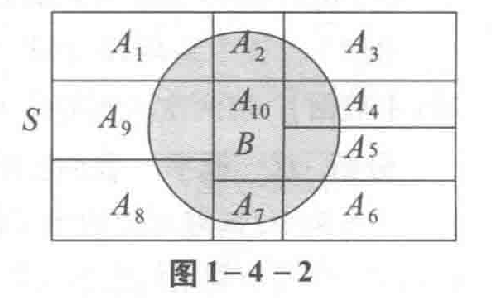
\includegraphics[scale=.5]{total_prob}
    \caption{全概公式示意图}
\end{figure}
\qs{P14-10}{
    从1到9的整数中有放回地依次随机抽取3次,求取出的3个数之积能被10整除的概率.
}
显然这三个数中必有两数为$5$和$\{2,4,6,8\}$,因此
\pf{法一}{
    分情况讨论
    \begin{enumerate}
        \item A = \{三个数里有两个5和一个偶数\}
        \item B = \{三个数里有一个5和两个偶数\}
        \item C = \{三个数里有一个5一个偶数和一个其他的奇数\}
    \end{enumerate}
    那么有
    \(\Pr{A} = \frac{\binom{4}{1}\cdot 3}{9^3}\)\,\,%
    \(\Pr{B} = \frac{\binom{4}{1}\cdot 3+\tbinom{4}{2}\mathrm{A_3^3}}{9^3}\)\,\,%
    \(\Pr{C} = \frac{\binom{4}{1} \binom{4}{1} \mathrm{A_3^3}}{9^3}\)%
    相加得\(\frac{156}{729}\).
}
\pf{法二}{
    对立事件\\
    不妨设三个数中出现$5$的事件为$A$,出现偶数的事件为$B$,那么
    \begin{align*}
        \Pr{AB} & = 1 - \Pr{\overline{AB}}                                                                   \\
                & = 1 - \left(\Pr{\overline{A}} + \Pr{\overline{B}} - \Pr{\overline{A}\,\overline{B}}\right) \\
                & = 1- \left(\frac{8^3}{9^3} + \frac{5^3}{9^3} - \frac{4^3}{9^3}\right)                      \\
                & = \frac{156}{729}
    \end{align*}
}
\pf{法三}{
    另一种分情况讨论(笔者的分法)
    \begin{enumerate}
        \item A = \{三个数中有两个相同的\}
        \item B = \{三个数全不同\}
              \reversemarginpar\marginnote[\footnotesize\color{red}\textbf{此项须要分成下述两项,否则会重}]{}
              \begin{enumerate}[label*=\arabic*.]
                  \item$B_1$ = \{三个数全不同且有两个偶数\}
                  \item$B_2$ = \{三个数全不同且有两个奇数\}
              \end{enumerate}
    \end{enumerate}
    那么有
    \(\Pr{A} = \frac{\binom{4}{1}\binom{3}{1}+ \binom{4}{1}\binom{3}{1}}{9^3}\)\,\,%
    \(\Pr{B_1} = \frac{\binom{4}{1}\binom{4}{1}\binom{3}{1}}{9^3}\)\,\,%
    \(\Pr{B_2} = \frac{\binom{4}{1}\binom{4}{1}\mathrm{A_3^3}}{9^3}\)%
    相加得\(\frac{156}{729}\).
}
\nt{
    讨论各种情况的概率进而求得所求事件的概率的方法实际上是\vocab{全概率公式}的一种体现.
}
\subsection{Beyes公式}
\vocab{全概公式}是通过计算某一事件会发生的\textbf{所有原因和情况的可能性大小}来计算该事件发生的概率,而\vocab{Beyes}公式则与之相反,考察一件已经发生的事情的\textbf{各种原因或或情况的可能性大小}.
\leftnote[1.8cm]{$\Pr{A_i}$,$\Pr{A_i|B}$分别称为原因的先验概率和后验概率}
\thm{Beyes公式}{
    设$A_1,A_2,\cdots,A_n$是一个完备事件组,且$\Pr{A_i} >0\,\textrm{for i in 1\dots{n}}$,则对任一可能发生的事件$B$,有
    \[\Pr{A_i|B}=\frac{\Pr{A_i}\Pr{B|A_i}}{\sum_{j=1}^{n}\Pr{A_j}\Pr{B|A_j}}\]
}
\section{事件的独立性}
\leftnote[1cm]{\textbf{独立与互斥是两种不同的概念}}
\dfn{两事件独立性}{
    设$A,B$是两个事件,若
    \[\Pr{AB}=\Pr{A}\Pr{B}\]
    则称$A,B$\vocab{相互独立}.
}
\thm{}{
    设$A$,$B$两事件相互独立且$\Pr{B}>0$,则有
    \[\Pr{A|B}=\Pr{A}\]
}
\thm{}{
    若$A$,$B$两事件相互独立,则它们对立事件和其本身(不同事件间)的组合也相互独立.
}

根据三个事件(略)独立性的定义,可以类推到n个事件的独立性:
设$A_1,A_2,\cdots,A_n$是$n$个事件,若对于其中任意$k(2\leq k\leq n)$个事件$A_{i_1},A_{i_2},\cdots,A_{i_k}$,有
\[\Pr{A_{i_1}A_{i_2}\cdots A_{i_k}}=\Pr{A_{i_1}}\Pr{A_{i_2}}\cdots\Pr{A_{i_k}}\]
则称$A_1,A_2,\cdots,A_n$\vocab{相互独立}.
\dfn{}{
    设$A_1,A_2,\cdots,A_n\,(n > 2)$是$n$个事件,若其中任意两个事件相互独立,则称这$n$个事件\vocab{两两独立}.
}
由此可以得到多个独立事件所具备的性质
\cor{}{
    设$A_1,A_2,\cdots,A_n\,(n > 2)$相互独立,则其中任意$k(2\leq k\leq n)$个(它们的对立)事件也相互独立.
}
\section{Bernoulli试验}
即两点分布.
\leftnote[1.8cm]{这相当于在实验结果序列中任取k次发生A事件}
\thm{Bernoulli定理}{
    一次试验中,事件$A$发生的概率为$p$,进行这样的试验n次,事件$A$发生$k$次的概率为
    \[b(k;n;p) = \binom{n}{k}p^k(1-p)^{n-k}\]
}
\nt{
n次Bernoulli试验的概率分布就是二项分布.其概率密度函数为
\[f(k,n,p)=\Pr(k;n,p)=\Pr(X=k)={\binom {n}{k}}p^{k}(1-p)^{n-k}\]
\textbf{Glossary}:两点分布=Bernoulli试验;二项分布=多次Bernoulli试验=Bernoulli概型.
}
\pf{辨析}{
    $\Pr{A}$ 和$\Pr(X)$使用的括号不同.大括号代表是事件,即一系列样本点集合(故而用大括号),小括号代表是随机变量(因为此时是概率密度函数).
}